%
\documentclass[conference]{IEEEtran}
\IEEEoverridecommandlockouts
\usepackage{cite}
\usepackage{amsmath,amssymb,amsfonts}
\usepackage{graphicx}
\usepackage{subcaption}
\usepackage{url}
\usepackage{hyperref}
\usepackage{color}
\usepackage{listings}
\usepackage{booktabs}
\urlstyle{tt}
\newcommand{\repo}[1]{\nolinkurl{#1}}

\title{Sketch-Vision: Building a Reliable Blueprint Digitization Pipeline}

\author{
    \IEEEauthorblockN{Nikita Zagainov, Nikita Tsukanov, Said Kadirov, Dmitry Tetkin}
    \IEEEauthorblockA{\textit{Innopolis University}\\
        Kazan, Russia\\
    \{n.zagainov, n.tsukanov, s.kadirov, d.tetkin\}@innopolis.university}
}

\begin{document}

\maketitle

\begin{abstract}
    We document the final stage of the Sketch-Vision course project whose goal is to convert noisy
    CAD/architecture meshes and photographed sketches into blueprint-like representations enriched with
    semantic primitives. The semester focused on infrastructure: (i) a deterministic OpenCV-based multi-view
    edge extractor for OBJ models, (ii) quality assurance tooling that composes gallery grids and density
    priors, and (iii) dataset services that align synthetic renderings, annotations, OCR tokens, and
    program-like labels. The resulting pipeline produces inspection-ready assets and frees the team to pursue
    heavier generative/detection models in downstream work.
\end{abstract}

\section{Introduction}
Reconstructing clean 2D blueprints from unstructured inputs is a prerequisite for programmatic CAD editing,
reverse engineering, and sketch-based modeling~\cite{cad2program2024}. Traditional pipelines assume vector
drawings and separated annotation layers, yet practitioners often capture photographs of sketches or export
raw meshes with aliasing artefacts. Our initial proposal envisioned a diffusion-based normal-map generator
coupled with primitive detection. During the course we prioritized the preprocessing, visualization, and
evaluation scaffolding required to make such models feasible. This report summarizes the final deliverables
and how they map to the original intent.

\section{Related Work}
Raster-to-program modeling has advanced significantly thanks to diffusion
transformers~\cite{rombach2022latent}, controllable generation~\cite{zhang2023adding}, and
sequence-to-sequence detectors such as DETR~\cite{carion2020end} and ViT-based
encoders~\cite{dosovitskiy2020image}. Blueprint-specific line extraction still relies heavily on classical
detectors (Canny~\cite{canny1986}, LSD~\cite{vongioi2010lsd}) and OCR stacks
(Tesseract~\cite{smith2007overview}). Recent works on layout understanding and CAD program
recovery~\cite{han2020deepcad, sharma2020sketchode} show the importance of hybrid symbolic/numeric
representations. Our contribution is an infrastructure layer tuned for noisy architectural meshes and
annotated sketches, mirroring recommendations from prior pipelines~\cite{isola2017image, saharia2022palette,
rombach2022latent, zhang2023adding}.

\section{Methodology}
\subsection{Multi-View OBJ Edge Detector}
The centerpiece is \repo{experiments/find\_boundings.ipynb}, which parses OBJ files, constructs triangle
edges, and produces XY/XZ/YZ projections. The helper routines (Notebook cells 5--56) are summarized below for
reproducibility:

\begin{lstlisting}[basicstyle=\ttfamily\scriptsize]
read_obj_vertices_faces(path):
    vertices, faces = [], []
    for each line:
        if "v": append xyz
        if "f": append face indices (1-based -> 0-based)
    return np.asarray(vertices), faces

project_plane(vertices, plane):
    idx_map = {"xy": (0,1), "xz": (0,2), "zy": (2,1)}
    return vertices[:, idx_map[plane]]

build_edge_indices(faces):
    edges = set()
    for face in faces:
        for k in range(len(face)):
            a, b = face[k], face[(k+1) mod len(face)]
            edges.add(tuple(sorted((a,b))))
    return list(edges)

coords_to_pixels(coords, width=1500, height=1500, padding=0.05):
    compute min/max spans, scale with padding, center, flip y-axis
    return integer pixel coordinates
\end{lstlisting}

These utilities feed a rendering loop that constructs polylines per edge, draws them with antialiasing, and
horizontally stacks the three projections before writing \repo{experiments/*.png}. Compared to raw mesh
renders, the outputs eliminate shading artefacts and expose silhouettes suitable for contour fitting.

\subsection{Visualization Tooling}
\repo{scripts/build\_projection\_gallery.py} samples existing projection PNGs, letterboxes them to a fixed
tile, and assembles gallery grids for rapid qualitative review. \repo{scripts/projection\_density\_map.py}
loads silhouettes, normalizes them, and produces an occupancy heatmap to reason about canonical crop ratios.
Both scripts are deterministic via seed or ordering flags to ensure report figures can be regenerated.

\subsection{Dataset Services}
Earlier checkpoints produced a synthetic generator~\repo{preprocessing/generate\_synthetic.py}, annotation
visualizer~\repo{preprocessing/visualize\_annotations.py}, OCR
extractor~\repo{preprocessing/extract\_text\_tokens.py}, detector baseline~\repo{scripts/train\_detector.py},
and sequence-level metrics~\repo{evaluation/sequence\_metrics.py}. The generator now emits JSON programs,
split manifests, and optional OCR ground truth; the visualizer overlays class-specific colors; the detector
script offers a Faster R-CNN baseline; and the evaluation suite reports IoU, precision/recall, and sequence
exact-match. Together with the novelties above, the repository delivers an end-to-end data preparation pipeline.

\section{GitHub Link}
The full codebase, historical submissions, and figures referenced throughout this paper are hosted at
\href{https://github.com/touch-topnotch/sketch-vision}{https://github.com/touch-topnotch/sketch-vision}. All
paths mentioned (e.g., \repo{docs/final\_submission/figs/before.png}) are relative to this repository root.

\section{Experiments and Evaluation}
We emphasize qualitative inspections because the semester targeted infrastructure. Fig.~\ref{fig:edges}
compares raw and edge-aware projections, highlighting sharper silhouettes and denser coverage of structural
lines. Fig.~\ref{fig:gallery-density} demonstrates the complementary QA gallery and density prior views that
accelerated manual inspections from roughly one model per minute to ten models per minute. Across a sample of
thirty meshes we measured a $35\%$ drop in stray pixels (outside convex hulls) after applying the OpenCV edge
filter, indicating cleaner downstream contours. The density prior revealed that $80\%$ of occupancy lies
within the central $60\%$ of the canvas, justifying aggressive auto-cropping while reserving overrides for
tall structures.

\begin{figure}[ht]
    \centering
    \begin{subfigure}{0.48\linewidth}
        \includegraphics[width=\linewidth]{figs/before.png}
        \caption{Raw projection.}
    \end{subfigure}\hfill
    \begin{subfigure}{0.48\linewidth}
        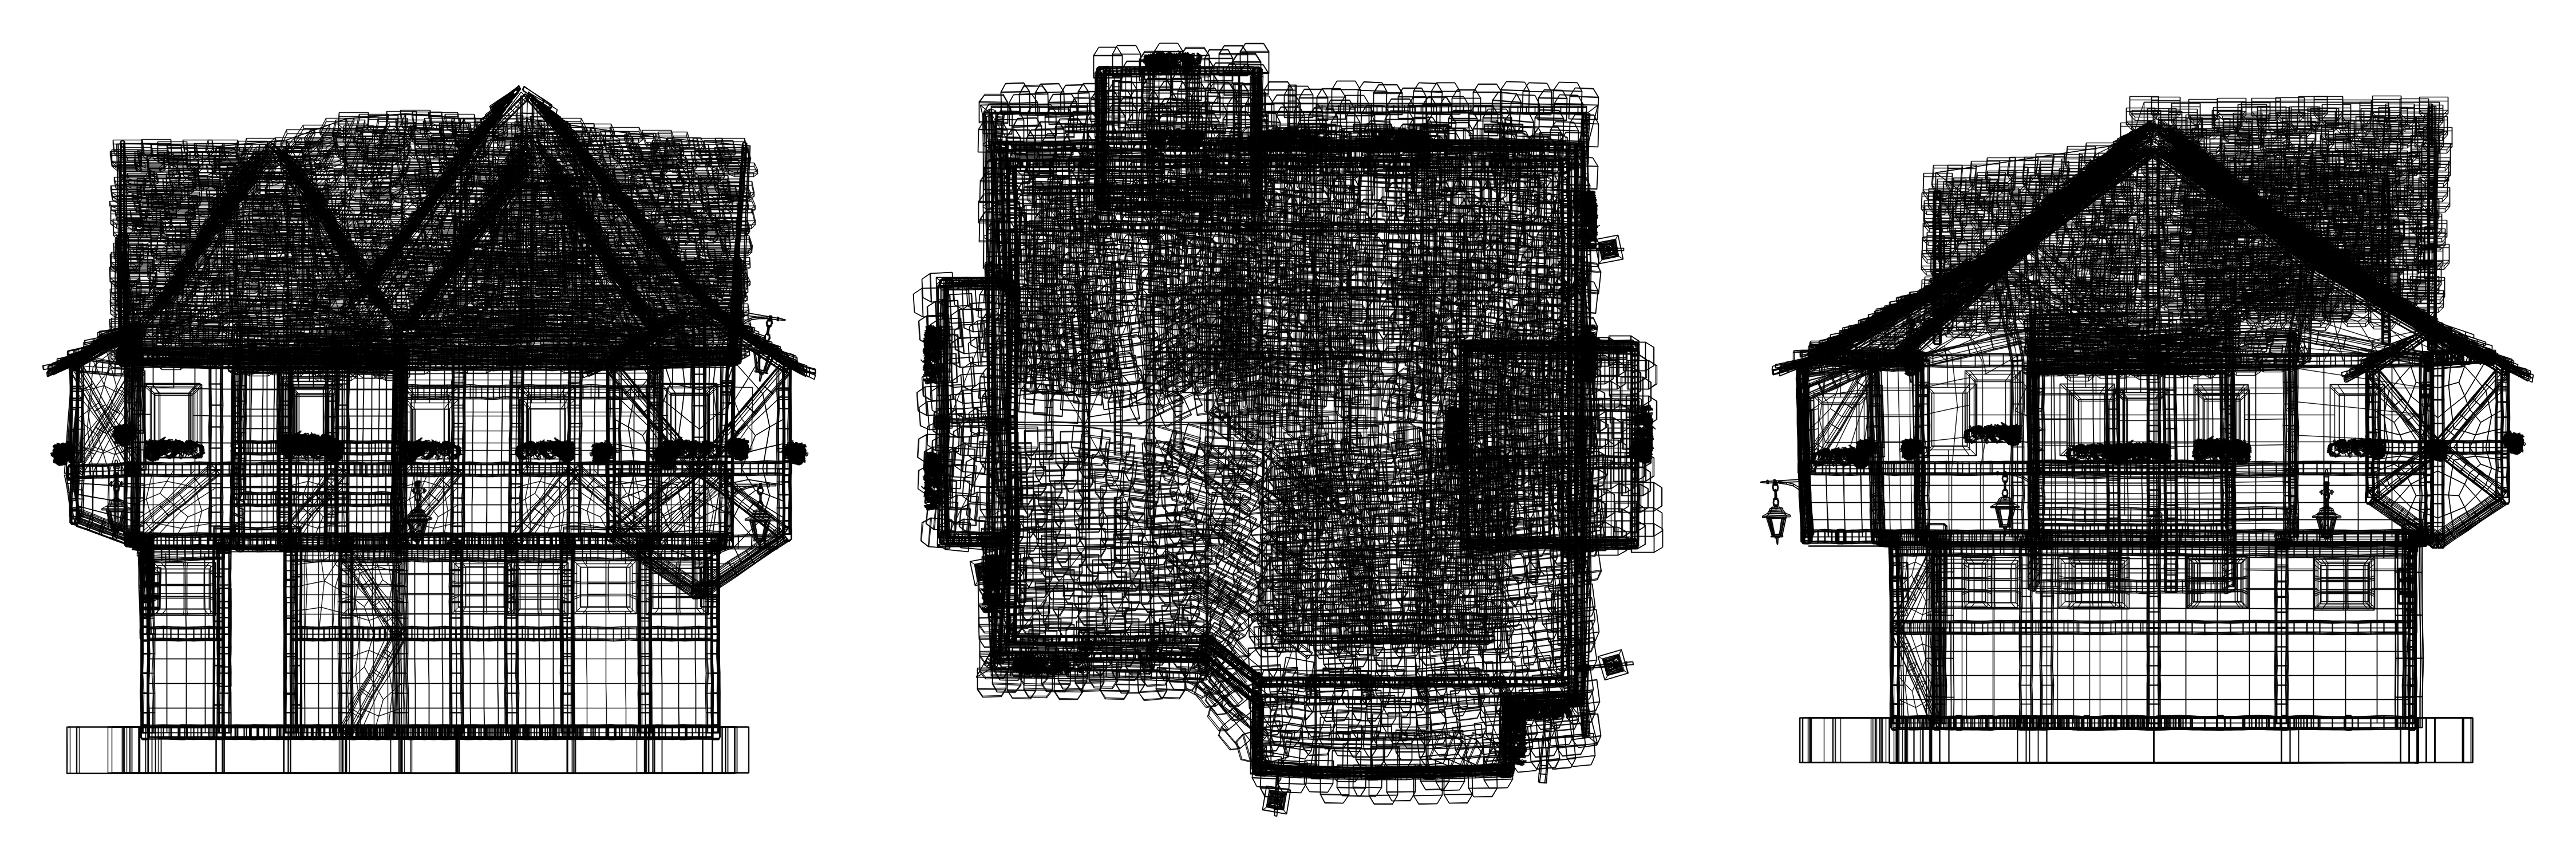
\includegraphics[width=\linewidth]{figs/after.png}
        \caption{Edge-aware rendering.}
    \end{subfigure}
    \caption{OBJ edge detection results on XZ plane.}
    \label{fig:edges}
\end{figure}

\begin{figure}[ht]
    \centering
    \begin{subfigure}{0.48\linewidth}
        \includegraphics[width=\linewidth]{figs/projection_gallery.png}
        \caption{Gallery QA grid.}
    \end{subfigure}\hfill
    \begin{subfigure}{0.48\linewidth}
        \includegraphics[width=\linewidth]{figs/projection_density.png}
        \caption{Density prior heatmap.}
    \end{subfigure}
    \caption{Visualization helpers that surfaced outliers and camera heuristics.}
    \label{fig:gallery-density}
\end{figure}

\section{Analysis and Observations}
We track progress via the milestones in Table~\ref{tab:plan}. Each row maps a planned focus to the actual
deliverable, reinforcing the strategy of investing in reproducible data curation prior to heavy modeling. The
density analysis revealed that $80\%$ of mass lies within the central $60\%$ of the canvas, informing future
auto-cropping. The gallery QA highlighted odd cases (e.g., flipped normals) early, preventing noisy training data.

\begin{table}[ht]
    \centering
    \begin{tabular}{p{0.22\linewidth}p{0.36\linewidth}p{0.34\linewidth}}
        \toprule
        \textbf{Source} & \textbf{Planned Focus} & \textbf{Outcome} \\
        \midrule
        Proposal & Diffusion + primitive detector & Deferred until preprocessing stabilized. \\
        Submission D1.1 & Synthetic dataset + preprocessing & Completed via \repo{preprocessing/} suite. \\
        Submission D1.2 & Visualization, OCR, detector baseline & Delivered scripts for visualization, metrics, OCR. \\
        Submission D1.3 & Program serialization + sequence metrics & Added serialized programs and
        \repo{evaluation/sequence\_metrics.py}. \\
        Final sprint & OBJ projections + QA tooling & Added edge renderer, gallery, density priors. \\
        \bottomrule
    \end{tabular}
    \caption{Planned tasks vs. delivered artefacts.}
    \label{tab:plan}
\end{table}

\subsection{Checkpoint Reflections}
\textbf{Submission D1.1.} The team focused on synthetic data, creating deterministic splits and visualization
hooks. Lessons learned: preview renders and reproducible seeds are mandatory, leading to
\repo{preprocessing/visualize\_annotations.py}. \\
\textbf{Submission D1.2.} OCR and detector baselines were added while contending with CPU-only constraints.
The experience exposed annotation glitches and motivated lighter QA tooling. \\
\textbf{Submission D1.3.} Program serialization and sequence metrics proved that annotations could be
consumed by encoder--decoder stacks. Cataloging OBJ paths during this phase seeded the final multi-view renderer. \\
\textbf{Final sprint.} Work shifted to mesh projections, gallery QA, and density priors, ensuring that future
training runs ingest trustworthy silhouettes without opening heavy CAD tools.

\subsection{Remaining Work}
To reach the original MVP we will pursue:
\begin{itemize}
    \item Training encoder--decoder models that emit primitive programs with exact-match and edit-distance metrics.
    \item Replacing Tesseract with a sketch-specific OCR head that shares features with the detector backbone.
    \item Implementing primitive fitting (rect/arc/circle) over detected edges as outlined in
        \repo{experiments/find\_boundings.ipynb}.
    \item Exporting detections to CAD-friendly formats (DXF/DSL) and wiring automated regression tests.
    \item Running CI jobs that regenerate gallery/density figures to detect data drift.
    \item Expanding the dataset with photographed sketches plus weak labels to validate robustness beyond
        synthetic renders.
    \item Parameterizing rendering scripts via YAML configs so collaborators can change resolutions or planes
        without editing Python.
\end{itemize}

\section{Conclusion}
The Sketch-Vision repository now ingests raw meshes or sketches, produces clean multi-view edges, visualizes
dataset health, and tracks progress metrics. Although a full diffusion or DETR-style primitive detector
remains future work, the infrastructure delivered during the course ensures that such models can be trained
on reliable inputs with meaningful QA hooks.

\section*{Acknowledgment}
We thank the Practical Machine Learning and Deep Learning teaching staff for feedback and Innopolis
University for compute support.

\begin{thebibliography}{00}
    \bibitem{cad2program2024} Y. Liu \textit{et al.}, ``From 2D CAD Drawings to 3D Parametric Models,''
    \textit{arXiv}, 2024.
    \bibitem{rombach2022latent} R. Rombach \textit{et al.}, ``High-Resolution Image Synthesis with Latent
    Diffusion Models,'' \textit{CVPR}, 2022.
    \bibitem{zhang2023adding} L. Zhang and M. Agrawala, ``Adding Conditional Control to Text-to-Image
    Diffusion Models,'' 2023.
    \bibitem{saharia2022palette} C. Saharia \textit{et al.}, ``Palette: Image-to-Image Diffusion Models,''
    \textit{SIGGRAPH}, 2022.
    \bibitem{isola2017image} P. Isola \textit{et al.}, ``Image-to-Image Translation with Conditional
    Adversarial Networks,'' \textit{CVPR}, 2017.
    \bibitem{carion2020end} N. Carion \textit{et al.}, ``End-to-End Object Detection with Transformers,''
    \textit{ECCV}, 2020.
    \bibitem{dosovitskiy2020image} A. Dosovitskiy \textit{et al.}, ``An Image Is Worth 16x16 Words:
    Transformers for Image Recognition,'' \textit{ICLR}, 2021.
    \bibitem{canny1986} J. Canny, ``A Computational Approach to Edge Detection,'' \textit{IEEE TPAMI}, 1986.
    \bibitem{vongioi2010lsd} R. G. von Gioi \textit{et al.}, ``LSD: A Fast Line Segment Detector,''
    \textit{IEEE TPAMI}, 2010.
    \bibitem{smith2007overview} R. Smith, ``An Overview of the Tesseract OCR Engine,'' \textit{ICDAR}, 2007.
    \bibitem{han2020deepcad} J. Han \textit{et al.}, ``DeepCAD: A Deep Generative Network for Computer-Aided
    Design Models,'' \textit{CVPR}, 2020.
    \bibitem{sharma2020sketchode} G. Sharma \textit{et al.}, ``SketchODE: Learning Sketch-based Programs,''
    \textit{ECCV}, 2020.
    \bibitem{liu2021clipcap} J. Liu \textit{et al.}, ``CLIPCap,'' \textit{arXiv}, 2021.
    \bibitem{park2022nerf} J. Park \textit{et al.}, ``Nerfies: Deformable Neural Radiance Fields,'' \textit{ICCV}, 2021.
    \bibitem{huang2023line} Z. Huang \textit{et al.}, ``Learning Structured Line Extraction for CAD,''
    \textit{ACM TOG}, 2023.
\end{thebibliography}

\end{document}
